\documentclass[bigger]{beamer}
\setbeameroption{show only notes}
\setbeamercolor{note page}{bg=white}
\setbeamercolor{note title}{bg=white}

\setbeamersize{text margin left=1cm, text margin right=1cm}
\setbeamertemplate{navigation symbols}{}
\setbeamertemplate{itemize items}{\textbullet}

\usepackage{graphicx}
\usepackage{helvet}
\renewcommand{\familydefault}{\sfdefault} % Sans-serif font like Arial
\setbeamerfont{frametitle}{size=\LARGE}
\setbeamerfont{framesubtitle}{size=\Large}
% \setbeamerfont{note page}{size=\footnotesize}

\setbeamertemplate{footline}{
  \leavevmode%
  \hfill
  
\includegraphics[height=0.5cm]{images/zengenti.png} % Adjust the height as needed
  \hspace{1em}
  \vspace{1em}
}

% \usebackgroundtemplate%
% {%
%   
\includegraphics[width=\paperwidth,height=\paperheight]{images/test_card.jpg}%
% }

\begin{document}
\title{All Code Sucks}
\subtitle{Why Bad Code is Everywhere and What to Do About It}
\author{Joe J Collins \\
  \href{mailto:j.collins@zengenti.com}{j.collins@zengenti.com} \\
  \href{https://linkedin.com/in/joejcollins}{linkedin.com/in/joejcollins}
}
\institute{
\includegraphics[height=1.5cm]{images/zengenti.png}}
\date{21 March 2024}

\begin{frame}[plain]
  \titlepage
  \note{I'm Joe Collins, I'm from Zengenti.\\
    We are a small company from Shropshire.\\
    About 70 nerds 
    We do websites for universities and local authorities.\\
    I don't actually do any websites, I work in the hosting team.\\
    We maintain the cloud on which the websites run.\\
    We use a combination of Ansible and Python\\
    to maintain an estate of about 3000 servers.\\
    However, tonight Matthew,\\
    I am going to talk about why all code sucks.\\
    \vfil
    We all know what good code looks like,\\
    or at least we think we do.\\
    But I should probably define what I mean by sucky code.\\
  }
\end{frame}

\begin{frame}{What is sucky code?}
  \framesubtitle{}
  \begin{quote}
    ``Programs are meant to be read by humans and
    only incidentally for computers to execute.''\\
    \hfill --- Donald Knuth
  \end{quote}
  \bigskip
  \begin{quote}
    ``It is better to have clean code that doesn't work
    than crap code that does.''\\
    \hfill --- Robert C. Martin
  \end{quote}
  \note{Don't take my word for it,\\
    Donald Knuth the Yoda of Computer Science\\
    says that code is for humans to read\\
    and sometimes for computers to run.\\
    He is all about the readability.\\
    \vfil
    Uncle Bob Martin in his inimitable style\\
    backs this up but uses the term clean code.\\
    But it is really a proxy for readability.\\
    If you and understand it then you can fix it,\\
    but if you can't understand it and it breaks you can't fix it.
  }
\end{frame}

\begin{frame}{The Great Hunt for Non Sucky Code}
  
\includegraphics[width=\textwidth]{images/companies.png}
  \note{I have been at this for about 25 years.\\
    Looking for code that doesn't suck.\\
    Trying to produce code that doesn't suck.\\
    I have worked with scumbags and saints.\\
    And in companies big and small.\\
    But all the code sucked.  Consistently.\\
    We did amazing things with it.  But it still sucked.
    \vfil
    Maybe I was just unlucky.\\
    But I have come to the conclusion that all code sucks.\\
    And that I should stop looking for the perfect code.\\
    And instead admit that all code sucks.\\
    And then work out what to do about it.\\
  Why does it all suck?}
\end{frame}

\begin{frame}{Why Code Sucks}
  \framesubtitle{The statistics favour suck}
  \begin{itemize}
    \item Half of everything is below average
      \pause
    \item Sturgeon's Revelation
      \pause
    \item The 2 Year Old Programmer Problem
  \end{itemize}
  \note<1>{
    Straight out of the gate, half of everything it below average.\\
    Well below the median.\\
  You don't have to be Francis Galton to realize that.}
  \vfil
  \note<2>{Then there is Sturgeon's law or revelation\\
    or whatever you want to call it.\\
    90\% of everything is shit.\\
    He was talking about science fiction at the time\\
    but it works in this situation.\\
    Only some things are really good.\\
  Put another way most stuff isn't that good.}
  \note<3>{
    Then an issue perculiar to the programming business,\\
    the demand for programmers over the last 25 years has always outstripped supply.\\
    When I started working the average working age was 2-3 years.\\
    And that hasn't changed.\\
    As more and more people have entered the business\\
    then have kept the average age down.\\
    There are a few old lags around but\\
    as a group we still don't have that much experience.
  }
\end{frame}

\begin{frame}{Why Code Sucks}
  \framesubtitle{Organisations tend to suck}
  \begin{itemize}
    \item Structure of Software Startups
      \pause
    \item Summer Student Projects
      \pause
    \item Prototypes in Production
      \pause
    \item The Agile Manifesto
      \pause
    \item New projects = New programmers
  \end{itemize}
  \note<1>{
    The architypal software startup is a couple of guys in a garage.\\
    In my experience this is true.\\
    We tend to romanticize Bill Gate and Steve Jobs.\\
    But it is a real thing.\\
    For most start ups the two guys are the dad and the son.\\
    The dad is the salesman.\\
    And the son is the programmer,\\
    who has been excluded from school for behavioural issues.\\
    They are not looking for books on best practice\\
    to read and contemplate.\\
    Turning to an authority is not on their agenda.\\
    The third employee?\\
  The son's best mate from school who was also excluded.}
  \note<2>{
    The other kind of startup that occurs in big companies.\\
    The summer student project.\\
    Alternatively called the unsupervised use of new technology.\\
    All the experienced programmers are on holiday or busy.\\
    So they give the new technology to the summer students to have a go.\\
  If it runs they put it into production.}
  \note<3>{
    Which brings us to another organisational imperative.\\
    Everyone agrees that the prototype will be thrown away.\\
    Then we will build the real thing.\\
    It never is.\\
    It is always put into production.\\
  And lives forever.}
  \note<4>{
    Then there is Agile
    I was there 25 years ago\\
    I was there the day the strength of Men failed\\
    and we deliberate misread the Agile Manifesto.\\
    We read `responding to change over following a plan'\\
    as `no need plan'.\\
  }
  \note<5>{
    New projects = New programmers.\\
    The NASA example.\\
    The average age of the team that helped get Neil Armstrong to the moon was 28.\\
    They were all new to the business.\\
  }

\end{frame}

\begin{frame}{Why Code Sucks}
  \framesubtitle{Psycho Suck}
  \begin{itemize}
    \item Availability bias
      \pause
    \item The Illusion of Explanatory Depth
      \pause
    \item Parkinson's Law of Triviality
      \pause
    \item The Lake Wobegon Effect
  \end{itemize}
  \note<1>{
    Availability bias.\\
    You only ever look at the bad code.\\
    You never look at the good code.\\
    You never look at the code that works.\\
    You only ever look at the code that doesn't work.\\
  So you think all code sucks.}
  \note<2>{
    The Illusion of Explanatory Depth.\\
    Everything is simple until you look.\\
    You think you know how it works.\\
    But you don't.\\
    You think you know how it works.\\
  But you don't.}
  \note<3>{
    Parkinson's Law of Triviality.\\
    Judging software design=nuclear reactor.\\
    We all think we are above average.\\
  We all think we are above average.}
\end{frame}

\begin{frame}{What Not To Do}
  \framesubtitle{}
  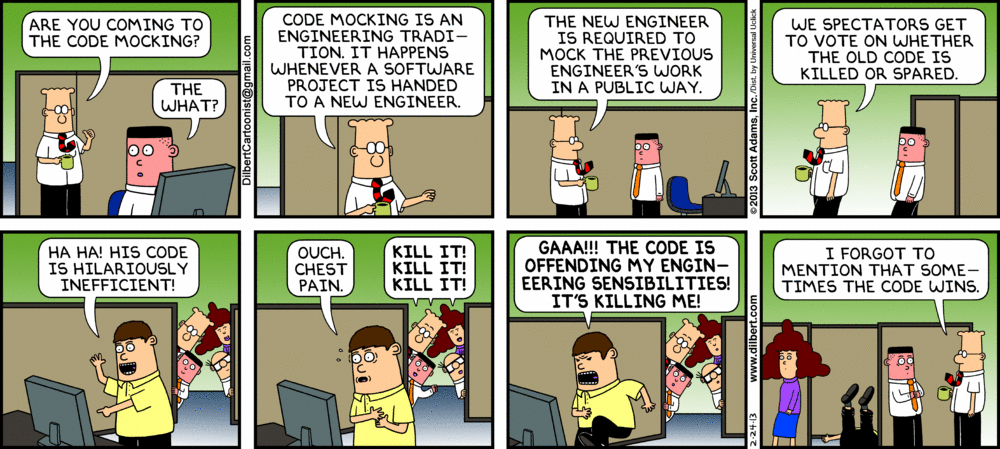
\includegraphics[width=\textwidth]{images/code-mocking.png}
  \note{So what not to do?\\
    Well so far railling against it hasn't helped.\\
    And Dilbert style mocking is positively harmful.\\
    Everyone is doing their very best\\
    with the time, resources and knowledge they have.\\
    If we assume the code will suck and we just have to work with it.\\
  Then we can start to work out what to do about it.}
\end{frame}

\begin{frame}{What To Do}
  \framesubtitle{Based on the work of Michael Feathers}
  \begin{itemize}
    \item Put the code in a vice (a test harness)
    \item Get ahead of the offending code with a feature flag
    \item Side by side rewrite
  \end{itemize}
  \note{
  }
\end{frame}

\begin{frame}{The Challenge}
  \framesubtitle{Where I need your help}
  \begin{quote}
    ``It's not that hard...''\\
    \hfill --- Billy Beane
  \end{quote}
  \bigskip
  \begin{quote}
    ``It's incredibly hard''\\
    \hfill --- Ron Washington
  \end{quote}
  \bigskip
  \note{To quote Moneyball,\\
    the challenge is both easy and difficult.\\
    Taken
  }
\end{frame}

\begin{frame}[plain]
  \centering
  {\Huge \bfseries Thank You!}\\[1cm]
  {\large Joe J Collins} \\[0.5cm]
  
\includegraphics[height=1.5cm]{images/zengenti.png}
\end{frame}

\end{document}
